\documentclass[11pt]{article} \usepackage{amsmath, amsthm, amssymb}
\usepackage{array,mathtools} \usepackage[textwidth=8in,textheight=9in]{geometry} %
\newcommand\showdiv[1]{\overline{\smash{\hstretch{.5}{)}\mkern-3.2mu\hstretch{.5}{)}}#1}} %
\newcommand\ph[1]{\textcolor{white}{#1}} %
\newcommand*{\carry}[1][1]{\overset{#1}} % \newcolumntype{B}[1]{r*{#1}{@{\,}r}}
\usepackage{listings} \usepackage{courier} \setlength{\oddsidemargin}{-1cm}
\setlength{\evensidemargin}{0cm} \setlength{\textwidth}{500pt}

\usepackage{color} \usepackage{wrapfig} \usepackage{url}

\usepackage{listings} \usepackage{color}

\definecolor{mygreen}{rgb}{0,0.6,0} \definecolor{mygray}{rgb}{0.5,0.5,0.5}
\definecolor{mymauve}{rgb}{0.58,0,0.82}

\usepackage{courier}

\lstset{basicstyle=\footnotesize\ttfamily,breaklines=true}
\lstset{framextopmargin=50pt,frame=bottomline}

\title{Mega Lit Review} \author{Luka Milic: lm1015}

\begin{document}
\maketitle
%
%
%
\section{Background}
\subsection{Introduction}
The aim of the project is to implement a
neural network which can take both labelled and unlablled face images.
\cite{tensorflow} This is relevant to the field of pattern
recogintion because real life is mainly unlabeled. Likewise most human
learning is also unsupervised\cite{Rocki2016}, hence it makes sense to try and create algorithms
which can some learning in an unsupervised way. This is called semi-supervised learning and is a active research field.

Semi-supervised algorithms in machine learning have been researched for a long
time, the focus here is on neural networks. So the first thing that comes to mind
is pre-training a network, one way to do this is with an autoencoder, which
pre-trains the weights in such a way to find useful representations of the data.
This is the line we will go down, the idea is to pass the unlabled data through
an autoencoder and then only use the encoding layer and an additional classification
layer for the final network.
%
%
%
\subsection{Theory}
Basic high level introudction
Gradients
Activation functions

{\bf Autoencoders}
Denoising
\newline Sparse
\newline Variational

%
%
%
\subsection{Related Work}
\subsubsection*{Andrew Ng autoencoder lecture notes}
This provids the nessecary background and also nicely
defines how to implement a sparse autoencoder. Sparsity constrains the average
activation of each neuron forcing the autoencoder to try to create even more
compressed representations of the data.
\subsubsection*{Shashank}
non-additive
effects of multiple AU's, non linear interaction

\subsubsection*{Amogh Gudi}
\cite{Gudi2015}

\subsubsection*{Jaiswal}
\cite{Jaiswal2016}
The 7 layer network is composed of 3 convolutional
layers and a max-pooling layer. The final fully connected layers provide the
classification output.
\subsubsection*{Deconvoltuional step in autoencoder} This is
a good paper \url{http://arxiv.org/pdf/1506.02753v4.pdf} and here is the
discussion I found it on
\url{https://www.quora.com/Deep-Learning-How-does-one-reverse-the-max-pooling-layer-for-reconstruction-in-the-decoding-part-of-an-auto-encoder}


\section{Progress Report}
%
%
%
\subsection{Datasets}
\begin{figure} \begin{center}
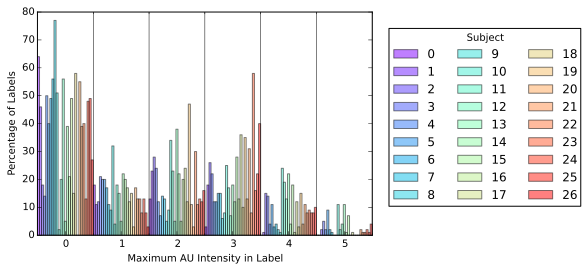
\includegraphics[width=1.0\textwidth]{../graphs/maximum_label_intensity_disfa.pdf} \end{center}
\caption{Basic structure of the network} \end{figure}


%
%
%
\subsection{Method}
\begin{figure} \begin{center}
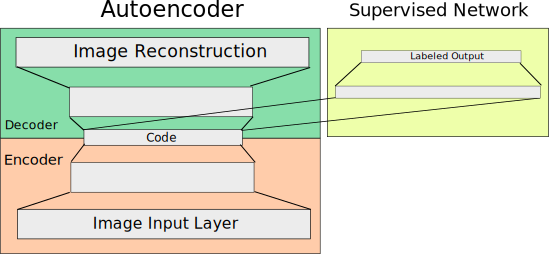
\includegraphics[width=0.5\textwidth]{illustrations/network_01.pdf} \end{center}
\caption{Basic structure of the network} \end{figure}
precision, recall, F1 score, ROC curve
%
%
%
\subsection{Results}
Here it would be nice to have proof I can detect AUs and an improvement with the autoencoder
%
%
%
\section{Plan}


\bibliographystyle{plain}
\bibliography{bib/autofaces}

\end{document}
